\documentclass[10pt,twocolumn]{article}
\usepackage[letterpaper,margin=.72in,top=.77in,bottom=.76in]{geometry}
\usepackage{amsmath,amssymb,booktabs,tabularx,array,graphicx,xcolor,tikz,microtype,hyperref,caption,fancyhdr}
\usetikzlibrary{arrows.meta,positioning,fit}
\definecolor{accent}{HTML}{146A72}
\hypersetup{colorlinks=true,linkcolor=accent,citecolor=accent,urlcolor=accent,pdftitle={MOSAIC: Source-Authoritative Generative Super-Resolution},pdfauthor={Shepherdess}}
\setlength{\columnsep}{.26in}
\setlength{\parindent}{1em}
\setlength{\parskip}{0pt}
\captionsetup{font=small,labelfont=bf}
\pagestyle{fancy}\fancyhf{}\fancyhead[L]{\small\textsc{MOSAIC}}\fancyhead[R]{\small Research preprint $\cdot$ v0.2}\fancyfoot[C]{\small\thepage}\renewcommand{\headrulewidth}{.3pt}
\title{\vspace{-1.2em}\textbf{MOSAIC: Model-Orchestrated Semantic Amplification via Image Compositing}\\[4pt]\large Source-Authoritative Generative Super-Resolution with Black-Box Image Editors}
\author{Shepherdess\\\small Independent research}
\date{24 November 2026 \quad $\vert$ \quad Research preprint, v0.2}
\begin{document}
\maketitle\thispagestyle{fancy}
\begin{abstract}
Generative super-resolution can improve perceptual detail while corrupting the geometry, identity, typography, and component topology of production assets. We present MOSAIC (Model-Orchestrated Semantic Amplification via Image Compositing), a backend-independent architecture that separates generative rendering capacity from authority over the assembled image. A deterministic Lanczos master anchors semantic crops and packed detail atlases, which are submitted to an external image editor with local constraints and global context. An explicit review gate precedes registered, selectively masked compositing. A declarative JSON protocol separates reusable method specifications, bound jobs, contract-addressed render records, and assembly reports. We document an executable Python implementation (protocol 1.1), derive its sequential compositing and illumination-correction equations, and distinguish these from a proposed normalized residual compositor. Eight synthetic tests reproduce five expected behaviors, including exact protected-raster and alpha preservation, and three implementation defects, including order-dependent overlap and incomplete cache integrity. No generative quality benchmark is claimed. We specify a controlled evaluation of detail, structural fidelity, cost, and incremental reuse. The contribution is an integrated, reproducible rendering architecture, not a new learned super-resolution network.
\end{abstract}
\noindent\textbf{Keywords:} super-resolution, image-to-image, semantic tiling, generative restoration, image compositing, fidelity, black-box inference.
\section{Introduction}
Single-image super-resolution (SR) is an underdetermined inverse problem. A low-resolution (LR) observation does not uniquely identify its high-resolution (HR) origin. Generative priors can supply plausible information about missing textures and edges, but realism and distortion are competing objectives \cite{blau}. For production assets, the costs of certain errors are asymmetric: an invented stitch may be acceptable, whereas a missing mechanical support or a changed letter can invalidate an otherwise attractive image.

General-purpose image-to-image editors offer a useful alternative to specialized SR networks because they can interpret the semantics of a region and accept natural-language constraints. However, a single full-image edit distributes finite output capacity over the entire scene. Fine components occupy few output pixels; an editor may redraw them rather than preserve them. A larger output resolution alone does not enforce fidelity.

MOSAIC borrows an engineering principle from multipass graphics rendering: allocate detail locally and retain global assembly authority outside the renderer. In contrast to treating a generated image as a replacement master, MOSAIC treats a generated region as a proposal whose contribution must be authorized. This creates a separation between \emph{rendering capacity} and \emph{image authority}.

The method is motivated by a practical attempt to enlarge an illustrated multi-view character reference sheet without changing its orthotic footwear, luminous hair, clothing, or typography. Independent rendering of overlapping component regions was proposed to concentrate the editor's capacity on detail, with the original retained as a registration and compositing reference.

\paragraph{Contributions.} We formalize (i) semantic, budget-aware selection of regional rendering tasks; (ii) an external, source-authoritative proposal and acceptance interface for arbitrary compatible image editors; (iii) bounded compositing with exact protected-region invariants and optional frequency-selective detail transfer; and (iv) a benchmark protocol measuring perceptual improvement, structural preservation, and cost. The accompanying implementation additionally introduces packed detail atlases, correction-aware assembly, declarative jobs and contract-addressed reuse. These are architectural contributions, not claims of a new learned SR model or demonstrated state-of-the-art performance.
\section{Related work}
\paragraph{Learned super-resolution and restoration.} Real-ESRGAN \cite{realesr} uses synthetic degradation modeling to train a practical blind SR network. SUPIR \cite{supir} applies a large generative prior to real-world restoration and uses fidelity-aware restoration mechanisms. SeeSR \cite{seesr} derives degradation-aware semantic conditioning to mitigate inaccurate content reconstruction. PURE \cite{pure} adapts an autoregressive multimodal model to perceive, interpret and restore degraded images. VOSR \cite{vosr} investigates vision-only generative SR. These approaches improve the restoration model itself; MOSAIC instead specifies an external inference architecture that can use such models or general-purpose image editors, where supported.
\paragraph{Regional diffusion.} MultiDiffusion \cite{multi} couples overlapping regional diffusion predictions during generation to produce a coherent result. Its fusion is performed within the iterative sampling process. PatchScaler \cite{patch} performs patch-independent SR with adaptive computation and is a close research precedent for spatially differentiated inference. MOSAIC does not require sampler access: its candidates are completed image outputs. It allocates output sampling density through cropping, and may separately allocate calls or retries based on region importance.
\paragraph{Tiled upscaling and local inpainting.} Ultimate SD Upscale \cite{ultimate} first enlarges an image, redraws tiles with padding, and offers seam-correction passes. ComfyUI Impact Pack \cite{impact} provides detector-driven detailers, and Inpaint CropAndStitch \cite{crop} already crops a masked area with context, resizes it for generation, and reinserts the result. These are the closest operational predecessors. MOSAIC does not claim novelty for crop, resize, inpaint, overlap, masking, or stitch operations in isolation. Its proposed research contribution is their organization around an immutable source, explicit structural acceptance rules, adaptive semantic resolution, independently reversible commits, and a black-box interface. Existing workflows can be extended to implement these same rules; the distinction is a testable system specification rather than an assertion of mutually exclusive capabilities.
\begin{figure*}[t]
\centering
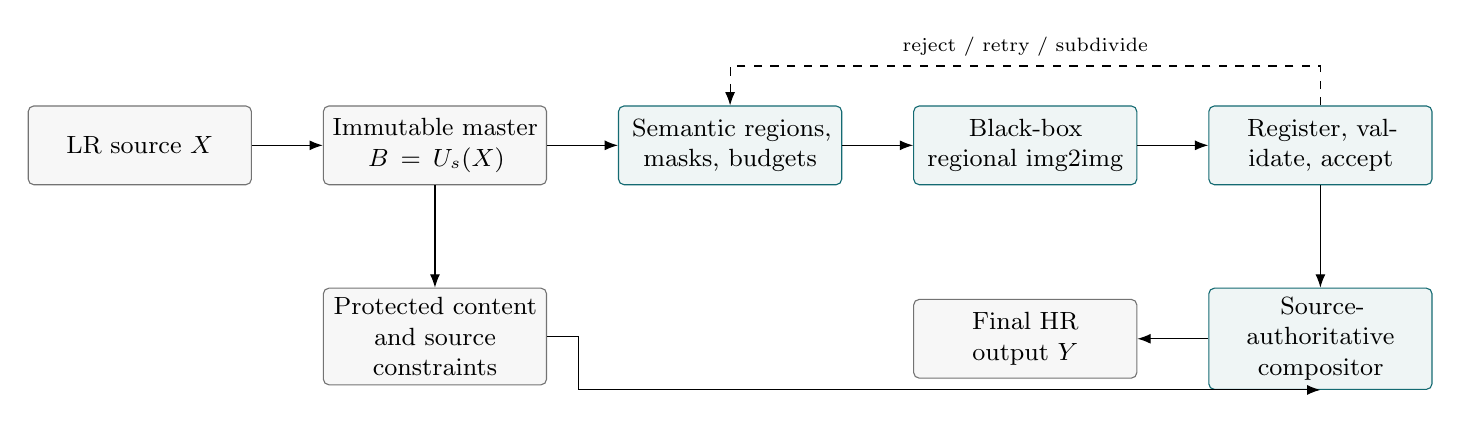
\begin{tikzpicture}[font=\small,>=Latex, node distance=9mm, every node/.style={align=center}, b/.style={draw=accent,rounded corners=2pt,fill=accent!7,minimum height=10mm,text width=26mm}, s/.style={draw=black!55,rounded corners=2pt,fill=black!3,minimum height=10mm,text width=26mm}]
\node[s] (x) {LR source $X$};
\node[s,right=of x] (base) {Immutable master $B=U_s(X)$};
\node[b,right=of base] (plan) {Semantic regions, masks, budgets};
\node[b,right=of plan] (render) {Black-box regional img2img};
\node[b,right=of render] (gate) {Register, validate, accept};
\node[b,below=13mm of gate] (merge) {Source-authoritative compositor};
\node[s,left=of merge] (out) {Final HR output $Y$};
\node[s,below=13mm of base] (protect) {Protected content and source constraints};
\draw[->] (x)--(base);\draw[->] (base)--(plan);\draw[->] (plan)--(render);\draw[->] (render)--(gate);\draw[->] (gate)--(merge);\draw[->] (merge)--(out);\draw[->] (base)--(protect);\draw[->] (protect.east)--++(4mm,0) |- (merge.south);\draw[->,dashed] (gate.north)--++(0,5mm)-|node[pos=.25,above,font=\scriptsize]{reject / retry / subdivide} (plan.north);
\end{tikzpicture}
\caption{MOSAIC architecture. Generators supply candidate regional detail; the immutable master and external acceptance/compositing stages retain final authority. Dashed path denotes bounded retries or subdivision.}
\label{fig:arch}
\end{figure*}
\section{Problem formulation}
Let $X\in[0,1]^{h\times w\times c}$ be a decoded source image and $s$ the desired linear enlargement factor. The target domain $\Omega$ has dimensions $H\times W$, where $H=sh$ and $W=sw$ (rounded as required). Let $B=U_s(X)$ be a deterministic interpolation of the source, e.g., Lanczos, stored in a fixed color space and bit depth. $B$ is immutable throughout inference.

A region plan consists of tasks $r_i=(C_i,M_i,p_i,b_i)$, where $C_i$ is a context crop, $M_i:\Omega\rightarrow[0,1]$ is the writable mask, $p_i$ is a component-specific constraint description, and $b_i$ is an inference budget. The support of $M_i$ lies within $C_i$. Context crops may overlap substantially even when writable interiors do not. A protected mask $P:\Omega\rightarrow\{0,1\}$ identifies pixels ineligible for generative replacement.

The objective is to improve local perceptual detail subject to source constraints and finite cost. Abstractly, choose candidates and compositing weights to maximize
\begin{equation}
Q(Y;X)-\lambda D(Y;X)-\mu\mathcal C,
\end{equation}
where $Q$ measures detail quality, $D$ source inconsistency, and $\mathcal C$ rendering cost. In practice these terms are not assumed to be reliable differentiable objectives; the pipeline uses explicit constraints and separate evaluation metrics. The hard protected-region constraint is
\begin{equation}
Y(u)=B(u)\quad\text{for all }u\text{ with }P(u)=1.
\label{eq:invariant}
\end{equation}
This guarantee concerns the decoded master raster, not unknowable original HR content. It is maintained by applying the protection mask at final assembly and exporting losslessly.
\section{Method}
\subsection{Semantic region planning}
A planner partitions the scene into meaningful parts such as faces, fabric panels, orthotic mechanisms, labels, or background. Regions may be specified manually, through segmentation, or by a multimodal planner. The plan records both the region's local semantics and dependencies crossing its boundaries. A knee hinge and its connecting struts, for example, should share a context crop or explicitly constrained landmarks even if their rendering passes are separate.

A region plan is not a partition of $B$. Context crops may overlap substantially, writable masks need not tile the canvas, and a component that straddles the boundary between two convenient rectangles is planned as a region in its own right, centred on the component, rather than being split between its neighbours. This is not a corner case: in the 2026-11-24 validation run on a multi-view character sheet, the fourth full-body view straddled the seam between two large rectangular sections, belonged fully to neither, and was absent from the assembled result---in one retry, an operator prompt that misdescribed its strip of the neighbouring section deleted it outright. The same run showed the dual failure: a single region containing three full-body views was large enough to ration rendering capacity exactly as a full image does, and one candidate collapsed all three views into a single zoomed view while still matching the region's aspect ratio. Region granularity is therefore a first-class planning decision: a region should hold few components, subdivision is the remedy for a crowded region (Section~\ref{sec:target-algorithm}), and dimensional agreement between a candidate and its region is not evidence of structural agreement---component counts are.

Regions are prioritized according to detail deficit, visual or functional importance, and structural risk. The planner can use an inexpensive initial SR estimate or human annotation to identify problem areas. Large simple backgrounds may be left at $B$; compact detailed regions can receive multiple full-resolution renders. Guard bands add context around writable interiors, reducing boundary uncertainty at the cost of some effective amplification.
\subsection{Output sampling density}
Let a full-image generation have output area $A_g$, and let a context crop cover fraction $f$ of the source area. If a crop is rendered at the same output area and aspect ratio is preserved, its approximate sampling density relative to full-frame rendering increases by
\begin{equation}
\rho_{\rm area}=1/f,\qquad \rho_{\rm linear}=1/\sqrt f.
\label{eq:density}
\end{equation}
For a crop occupying one sixteenth of the image, the idealized gain is $16\times$ in pixel allocation or $4\times$ in linear sampling density. Context padding, aspect-ratio fitting, model preprocessing, and final resampling reduce this gain. This is an allocation argument, not a guarantee of true detail recovery or information-theoretic resolution.

More generally, if a region crop has source dimensions $w_i,h_i$ and usable rendered dimensions $g_{wi},g_{hi}$, its local sampling scale is $\min(g_{wi}/w_i,g_{hi}/h_i)$. The planner targets at least $s$ before resampling and can subdivide when the editor's maximum usable output is insufficient. It avoids subdivision if the crop would lose essential semantic context.
\subsection{Black-box regional rendering}
For each task, the renderer receives a crop from $X$ or $B$, optionally the global source as an additional reference, and a prompt describing the desired refinement and prohibited changes. A backend need only expose an image-conditioned output interface:
\begin{equation}
Z_{ij}=G_j(\operatorname{crop}(X,C_i),p_i,\kappa_i),
\end{equation}
where $j$ indexes a candidate or backend and $\kappa_i$ denotes supported auxiliary context, settings, or references. An adapter maps these inputs to the actual backend. Global-reference support, reproducible seeds, and control over denoising are optional. No hidden states or gradients are required.

The default prompt preserves source pose, silhouette, topology, material identity, and lighting while requesting finer detail. Editing requests unrelated to enlargement should be represented as a separate explicit stage or as separately authorized masks. The renderer must not silently introduce such changes as part of SR.
\subsection{Registration and candidate validation}
Generated candidates may drift in placement, scale, or shape. Register each $Z_{ij}$ to its source footprint using the known crop mapping and, where necessary, robust feature correspondences or manually defined landmarks. Prefer similarity or affine transforms with bounded parameters. More flexible warps require separate justification and diagnostics, since they can conceal structural errors. A candidate without reliable correspondences is rejected or sent for review.

Let $R_{ij}$ be a registered candidate resampled to the target grid. A validator returns a binary acceptance decision $a_{ij}$ and optional spatial confidence $q_{ij}(u)\in[0,1]$. Acceptance is conditional on predeclared limits for landmark displacement, silhouette disagreement, source-scale consistency, protected-pixel intersections, and component-specific attributes. The source-scale check compares downsampled registered content against the corresponding source observation using an explicitly chosen degradation operator and mask. It can reveal substantial drift but cannot verify unobserved fine detail.

For structured assets, a component can be described by an attributed graph $\mathcal G_i=(V_i,E_i)$, with vertices representing joints, fasteners, or other required features and edges representing connections. A missing support, changed joint order, or new opening can be rejected even when a perceptual distance is small. Graph annotations may be manual. Automated detectors are fallible and should be calibrated against independent annotations. Multi-view sheets additionally permit cross-view checks of attributes expected to remain invariant across perspectives, not pixel-level equality of different views.
\subsection{Proposed normalized residual compositing}
Accepted candidates are combined as bounded residuals, not unconditionally substituted. For each region choose a registered candidate $R_i$ and define $D_i=R_i-B$ on its support. An optional frequency gate $\mathcal F_i$ limits the contribution to a high-frequency band, e.g., $\mathcal F_i(D_i)=D_i-L_\sigma(D_i)$ for a Gaussian low-pass filter $L_\sigma$. Filtering is performed on padded crops before masking. Color matching against the master may be applied before residual extraction. Full-band replacement is available where geometry and color changes are explicitly permitted.

Define $v_i(u)=a_i M_i(u)q_i(u)$, with feathering incorporated in $M_i$. Set $S(u)=\sum_i v_i(u)$ and $w_i(u)=v_i(u)/\max(1,S(u))$. The final composite is
\begin{equation}
Y=\operatorname{clip}\left[B+(1-P)\sum_i w_i\mathcal F_i(D_i)\right].
\label{eq:composite}
\end{equation}
The weights are nonnegative and sum to at most one. Pixels with no accepted proposal retain $B$. Equation~\eqref{eq:invariant} holds by construction after protected pixels are copied from $B$ following any color conversion. The normalized sum avoids accumulating unbounded residuals across overlapping proposals. Incompatible candidates are not blended merely because they overlap; conflict resolution selects a winner, reduces confidence, or retains the master. A frequency gate can reduce low-frequency color and shading drift, but does not independently guarantee edge or topology preservation.

For text and logos, MOSAIC defaults to a protected overlay sourced from $B$ or a separately authorized vector reconstruction. A vector rebuild is an edit, not evidence that original high-resolution lettering was recovered.
\subsection{Proposed transactional refinement}
Each accepted region is stored as a proposal record, including its crop, prompt, backend version, transform, validation data, mask and residual. Candidates are evaluated against $B$, not solely against previously generated neighbors. Global checks may invalidate an accepted region when conflicts emerge. Because the output is recomputed from $B$ and the retained proposal set, rollback is straightforward and commit order need not alter the result under a fixed conflict-resolution policy. A retry uses a revised prompt, increased context, alternate backend, or subdivision. The scheduler enforces a maximum call count and recursion depth; exhausted regions retain the base image.
\begin{table*}[t]
\centering\small
\caption{Comparison of representative approaches. Entries describe typical published or documented mechanisms, not all possible extensions.}
\label{tab:prior}
\begin{tabularx}{\textwidth}{@{}p{.17\textwidth}p{.24\textwidth}p{.24\textwidth}X@{}}
\toprule
Method & Regional allocation & Fidelity / assembly mechanism & Relationship to MOSAIC \\\midrule
Real-ESRGAN \cite{realesr} & Learned SR; optional implementation tiling & Trained degradation and reconstruction prior & Candidate backend or baseline \\
SeeSR / SUPIR \cite{seesr,supir} & Specialized generative restoration & Semantic conditioning / fidelity-aware restoration & Complementary model-level mechanisms \\
PURE / VOSR \cite{pure,vosr} & Multimodal or vision-only generative SR & Learned restoration formulation & Complementary generator-level mechanisms \\
MultiDiffusion \cite{multi} & Overlapping spatial diffusion paths & Fusion during iterative sampling & MOSAIC fuses completed proposals externally \\
PatchScaler \cite{patch} & Patch-independent adaptive inference & SR-specific diffusion pipeline & Closest academic precedent for adaptive allocation \\
Ultimate SD Upscale \cite{ultimate} & Padded grid tiles, redraw passes & Masked assembly and seam correction & Closest conventional tiled baseline \\
Impact Pack / CropAndStitch \cite{impact,crop} & Mask- or detector-selected crops & Local enlargement, regeneration, reinsertion & Closest operational precedent; can implement MOSAIC primitives \\
MOSAIC (this work) & Semantic crop allocation, optional recursion & Immutable master, structural acceptance, bounded residuals & External backend-independent orchestration \\
\bottomrule
\end{tabularx}
\end{table*}
\section{Target reference algorithm}\label{sec:target-algorithm}
\noindent\textbf{Inputs:} source $X$, target scale $s$, protection mask $P$, renderer adapter $G$, task and call budget $K$.\\
\textbf{Output:} composite $Y$, provenance manifest.
\begin{enumerate}\setlength{\itemsep}{1pt}
\item Construct immutable $B=U_s(X)$; initialize empty accepted proposal set $\mathcal A$.
\item Plan semantic regions, writable masks, guard bands, dependencies and local budgets.
\item While the task queue is nonempty and budget remains, choose a region by priority. Generate one or more candidates, accounting for each backend call.
\item Register candidates to $B$; run local geometry, source-consistency and semantic checks. Reject invalid candidates. Retry or subdivide only within the remaining budget.
\item Select a passing candidate using a declared ranking rule. Record its confidence, mask, residual and metadata in $\mathcal A$.
\item Resolve overlapping conflicts and cross-region or cross-view constraint violations; roll back affected candidates as needed.
\item Recompose using Eq.~\eqref{eq:composite}; restore protected pixels; export losslessly with the manifest.
\end{enumerate}
The algorithm above specifies the target architecture. The released protocol 1.1 executor implements a subset, with manual review, sequential alpha blending, bounded optical flow and explicit render records, as described next.

\paragraph{Compute and memory.} With $N$ tasks and $k_i$ candidates per task, total generation calls are $\sum_i k_i\le K$. Independent regional renders can be parallelized if backend limits permit. The compositor can process sparse residual footprints rather than full-size arrays; its work is approximately proportional to the target canvas plus the summed candidate footprint areas. MOSAIC may cost more than one global render and should be evaluated at matched quality and matched budget, not described as inherently faster. The benefit is controllable allocation and the ability to skip or rerender individual parts.

\section{Executable reference implementation}
The supplied protocol 1.1 package contains the reusable method manifest, a JSON Schema (Draft 2020-12), a blank job template, a workflow brief, an agent skill, construction-review guidance, and \texttt{scripts/sections.py}. The executable prepares crops and assembles accepted externally generated images; it makes no image-generation API calls. The planner and renderer may therefore be human-operated or agent-operated. The implementation prepares crops directly from the decoded source; the Lanczos target master is constructed at assembly time. This is equivalent to retaining a deterministic master as an authority, but not to cropping an already enlarged master for all inputs.

\subsection{Declarative rendering and reuse}
Four artifact types define the interface (Table~\ref{tab:artifacts}). A job binds the source path, integer scale, source-space rectangles with exclusive right and bottom edges, protected rectangles, section invariants, and optionally authorized corrections. Each section has either one rectangle or an atlas of multiple cells. The executor validates the job, checks source identity and coordinate bounds, and writes the prepared images and render records. An external operator submits each crop with the full source as context, where the backend supports it, and records the returned path and review decision. The executor enforces the recorded acceptance flag, not the semantic judgment itself.
\begin{table}[h]
\centering\small
\caption{Protocol 1.1 artifact roles.}\label{tab:artifacts}
\begin{tabularx}{\columnwidth}{@{}p{.33\columnwidth}X@{}}
\toprule Artifact & Function \\\midrule
Method manifest & Reusable procedure, defaults and reference roles \\
Bound job & Source, target, sections, protected content, corrections \\
Render records & Crop/atlas mappings, contract digests, render paths and acceptance \\
Assembly report & Output size, source digest, correction IDs, registration and local source error \\\bottomrule
\end{tabularx}
\end{table}
Let $h_X$ denote the SHA-256 digest of the source file. For section $i$, the implementation calculates
\begin{equation}
h_i=\operatorname{SHA256}(\operatorname{canon}(h_X,S_i,K_i)),
\end{equation}
where $S_i$ contains the selected geometry, input layout, invariants, prompt overrides and reference descriptors; $K_i$ contains job-level reference descriptors and corrections assigned to the section. Canonicalization uses JSON with sorted keys and compact separators. The job render contract hashes the source, intent and ordered section IDs and hashes. During preparation, matching section digests preserve accepted paths and review fields; differing digests invalidate acceptance. Previous record snapshots are archived when the aggregate digest changes. Assembly-only fields such as feathering can be changed without generating new imagery. This is an incremental compilation analogy: reuse a proposal when its declared rendering dependencies remain unchanged. The current hash coverage is incomplete, as demonstrated below; this is not a fully content-addressed cache.

\subsection{Generative atlasing and sampling density}
Multiple discontinuous detail crops may share a regular atlas. The executor packs each crop into a cell with a nominal four-pixel border on each side, using aspect-preserving Lanczos fitting. It records each actual placement rectangle. For atlas input dimensions $(I_w,I_h)$ and returned dimensions $(G_w,G_h)$, a cell with input placement width $a_w$ and height $a_h$ receives approximately $g_w=a_wG_w/I_w$ and $g_h=a_hG_h/I_h$ output pixels (before integer rounding). For source cell dimensions $(w,h)$, the conservative local linear allocation is
\begin{equation}
\rho_i=\min\left(\frac{a_wG_w}{I_ww},\frac{a_hG_h}{I_hh}\right).
\end{equation}
The executor rounds transformed cell boundaries, extracts each output independently and resizes it to the target footprint. Individual rectangle inputs are resized to a nominal long edge of 1536 pixels, with enlargement capped at $4\times$. Atlas padding and fitting reduce effective allocation. Atlasing amortizes call overhead at the potential cost of cross-cell interference and less local rendering capacity. It assumes the editor retains atlas layout; misplaced cells must be rejected. The paper's planner may optimize packing or recursively allocate renders; neither is automated in the supplied helper.

\subsection{Construction-first acceptance and corrections}
The review specification checks connectivity, component counts, orientation, occlusion, silhouette, identity and material continuity before fine finish. The review is repeated after alignment and assembly. A visually attractive but mechanically invalid candidate must be rejected rather than disguised by blending. The schema distinguishes \texttt{upscale\_only} from \texttt{upscale\_with\_corrections}, with named correction instructions scoped to section IDs. For the latter, matching and registration default to disabled in affected sections unless overridden, so the original geometry and color are not inadvertently restored over the intended change. Protected rectangles still take precedence. The correction list expresses authorization but does not automatically prove that the generated edits comply.

\subsection{Implemented compositor}
For a returned tile $R_i$ mapped to the target footprint, the optional OpenCV DIS optical flow routine estimates source-to-render displacement on a bounded working raster, smooths the field and clips vector magnitudes to a nominal eight source pixels by default. The field is rescaled to output coordinates for remapping. Clipping limits displacement but does not prove structural correctness. Broad illumination matching then approximates
\begin{equation}
\widehat R_i=\operatorname{clip}[R_i+\alpha_i(L_\sigma(B_i)-L_\sigma(R_i))],
\label{eq:implementedcolor}
\end{equation}
where $B_i$ is the separately resized source crop, $L_\sigma$ is a Gaussian blur with nominal radius $12s$ target pixels, and $\alpha_i=0.45$ for ordinary sections by default (zero for corrected sections). In ideal linear arithmetic before clipping, quantization and blending, this preferentially retains high-frequency detail while attenuating broad residual drift. Pillow performs the actual operation on encoded, quantized RGB values; the identity is an approximation to that implementation.

Let $m_i$ be the smoothstep edge-feather mask, optionally multiplied by a blurred polygonal edit mask. The implementation uses sequential masked paste rather than Eq.~\eqref{eq:composite}:
\begin{equation}
Y_i=(1-m_i)Y_{i-1}+m_i\widehat R_i,\quad Y_0=B.
\label{eq:sequential}
\end{equation}
Operations are applied to RGB with 8-bit mask rounding. Default feather widths are 12 source pixels for rectangles and 5 for atlas cells. After all pastes, protected rectangles are copied from the master, and nonopaque source alpha is replaced with the exact master alpha channel. A lossless PNG export therefore supports Eq.~\eqref{eq:invariant} for protected rectangles. Unlike the normalized residual formulation, Eq.~\eqref{eq:sequential} is order-dependent in overlaps. Unaccepted sections currently block assembly instead of falling back automatically to the master.

\section{Reproducible executor validation}
We executed eight unit tests on the supplied, unchanged protocol 1.1 executor. The synthetic fixture is a $48\times32$ RGBA gradient, enlarged to $96\times64$, with a rectangle and an overlapping atlas cell, distinct solid-color candidate renders, and a protected rectangle. One cache test uses an opaque version of the fixture. Alignment is disabled to isolate composition. Tests run locally using Python, Pillow 12.3.0 and NumPy 2.3.5. They require no remote model, credentials or network. The companion \texttt{tests/test\_executor.py} constructs the fixtures, and \texttt{tests/results.txt} records the run. All eight assertions passed; three deliberately reproduce defects rather than establish desired behavior.
\begin{table}[h]
\centering\small
\caption{Synthetic executor observations; not image-quality benchmarks.}\label{tab:tests}
\begin{tabularx}{\columnwidth}{@{}Xp{.26\columnwidth}@{}}
\toprule Observation & Result \\\midrule
Output dimensions, exact protected RGBA, alpha and untouched exterior & Confirmed \\
Cache reuse and selective invalidation after invariant change & Confirmed \\
Assembly-only feather change retains acceptance & Confirmed \\
Unaccepted section blocks assembly & Confirmed \\
Correction defaults disable color matching & Confirmed \\
Reversing overlap order changes output & Defect reproduced \\
Atlas background change leaves contract hash unchanged & Defect reproduced \\
Accepted render bytes can change without renewed review & Defect reproduced \\\bottomrule
\end{tabularx}
\end{table}
These checks establish narrowly scoped executor properties and provide regression targets. They do not measure perceptual improvements or the accuracy of a generator or visual validator. The optical-flow path and real generative candidates were not tested here.

\paragraph{Implementation roadmap.} Extend hashes to prepared input bytes, atlas background, reference contents, renderer and prompt versions, and accepted output bytes. Bind review decisions to immutable proposals and record structured review evidence. Introduce normalized conflict-aware residual blending, optional fallback to the master, explicit confidence fields, deformation diagnostics, and recursive budget scheduling. Preserve corrected regions against inappropriate source matching. These are proposed changes; the archived executor is unmodified. A normalized sum is order-independent only for a fixed candidate and weight set with deterministic conflict resolution. Neither a digest nor a passing visual review establishes factual recovery of missing detail.
\section{Motivating case study}
The motivating asset is a multi-view character reference sheet for Neon Night, featuring glowing blue hair and fur, dark clothing, articulated orthotic footwear and labels. The original task sought enlargement without full-image reconstruction. The artist identified detail loss in the boots and errors in whole-image regeneration, including conflation of front and rear boot features, incorrect open-heel interpretations of solid hollow platforms, and the risk of disappearing supports between the upper boot and knee hardware.

A regional rendering workflow was proposed on 23 November 2026: render overlapping sections at the generator's available output resolution, preserve the original as a registration reference, merge region interiors and seams, and composite lettering independently. The analogy was to console rendering techniques that allocate detail locally while retaining a coherent scene. This case motivates, rather than establishes, the formal method above.

\paragraph{Illustrative task plan.} Separate tasks would address hair/fur texture, jacket and fasteners, orthotic assemblies and footwear, and noncritical background. Each orthotic task would include the knee hinge, connecting struts and platform where needed for context. Annotated cross-view attributes would include support connectivity, hinge location, platform enclosure and lace routing. Typography and silhouettes that must not move would be protected. The initial source, regional candidate images and final composite should be retained for later analysis. The supplied case note records a 1536 by 1024 source and a target of 6144 by 4096. It reports improved eyelets, laces and reflections in a boot crop, followed by identification of missing bracing. Authenticated before/after pairs and quantitative measurements from that session are not included; no superiority claim is made from it.
\section{Evaluation protocol}
\subsection{Dataset and test strata}
Evaluate paired and unpaired SR at $2\times$ and $4\times$ using fixed, licensed or author-owned test images. A proposed initial test set contains 120 HR assets, stratified equally across natural photos, illustrations, typography-bearing diagrams, and multi-view or mechanical reference assets. Publish image identifiers, source licenses, degradation code, test splits and annotations. For paired tests generate LR inputs from known HR originals using deterministic downsampling and a second predefined blur/noise/JPEG degradation regime. Reserve a separate set for tuning thresholds. Add real LR images without HR ground truth to assess practical performance without claiming recovery accuracy.

\subsection{Baselines and ablations}
Compare Lanczos, Real-ESRGAN, a specialized generative SR baseline (e.g., SeeSR or SUPIR), Ultimate SD Upscale, and a crop-and-stitch detailer with comparable settings. The most important controlled comparison uses the \emph{same} general-purpose image editor for full-image rendering, uniform overlapping crops, semantic crops with simple blending, and full MOSAIC. Keep output dimensions, permitted modifications, and prompt intent fixed. Match generation call counts or measured cost and report quality--cost curves for unequal budgets. Where API models prevent exact replication, preserve the actual returned candidate images and request metadata.

Ablate semantic partitioning, guard bands, global-reference conditioning (where supported), registration, structural acceptance, frequency gating, recursion, and final source protection. Change one factor at a time and report interactions between protection and acceptance. Record the proportion of unchanged pixels so apparent fidelity cannot be attributed solely to leaving the input unmodified. Compare atlas packing with independent crops at matched cost; measure effective cell allocation, layout failures, acceptance rates, and rerender counts. For incremental workloads, perturb one invariant, one reference, one crop geometry, and one assembly setting at a time, recording invalidated sections, call savings and stale reuse. For corrective jobs, measure successful authorized changes separately from unrequested drift.
\subsection{Metrics}
\textbf{Paired fidelity:} PSNR, SSIM, LPIPS \cite{lpips} on aligned HR targets. Report both full-frame and annotated-region values. \textbf{Source consistency:} mean absolute error after a declared LR degradation operator; pixel equality on $P$; landmark displacement normalized to object size; silhouette IoU. \textbf{Semantic integrity:} count missing or spurious required components, graph edge errors, OCR character error rate, and cross-view attribute violations. \textbf{Seams:} compare gradient discontinuities in overlap bands with corresponding source and non-seam bands. \textbf{Perceptual quality:} blinded pairwise judgments at native output scale for detail quality and source faithfulness as separate questions. \textbf{Efficiency:} calls, retries, latency, billed cost, acceptance rate and modified area. Report failure rates and rejected cases, not just successful examples.

\subsection{Analysis plan}
Use paired differences per source image, stratified summaries, and image-level bootstrap confidence intervals; treat repeated candidates from one source as dependent observations. Use at least three independent generation runs where possible to characterize stochastic variation. Randomize human comparison order and blind method labels; use at least three independent ratings per pair. Predeclare the thresholds and primary endpoints before the test run. A candidate success criterion is improved human-rated detail relative to the same-backend uniform crop baseline, with no increase beyond a predeclared noninferiority margin in structural errors at matched cost. Establish the margin using domain-specific annotation tolerance on the development set. Report exact protection separately as an invariant rather than a statistical improvement.

\section{Limitations and discussion}
MOSAIC cannot reconstruct information uniquely absent from the source. It synthesizes plausible detail and rejects observable inconsistencies; it is unsuitable as evidentiary enhancement unless synthetic modifications are explicitly identified. The approach may fail on very small or ambiguous components, conflicting views, insufficient local context, and images with long-range patterns. Segmentation and registration introduce additional failure modes. A conservative validator may reject genuine improvements, while an overly permissive validator may approve convincing hallucinations. High-pass extraction can preserve unwanted artifacts or produce ringing. Higher call counts and API variability can limit throughput and reproducibility.

The architecture is not tied to a fixed image size or a particular diffusion implementation. It resembles a rendering graph whose nodes are generative proposals and whose compositor is the authority. The main research hypothesis is that this division of responsibilities yields a better detail--fidelity tradeoff for structured images than unconstrained full-frame generation or equally budgeted conventional regional workflows. Demonstrating that claim requires the comparative protocol above. Existing toolchains may reproduce the topology; the novelty claim is confined to the specified integration and its evaluation, pending broader prior-art review.
\paragraph{Two layers, two disciplines.} The architecture separates a deterministic layer from a generative one, and the 2026-11-24 experiments suggest each obeys an opposite discipline. The deterministic layer is linear, cheap and global, so it should run \emph{monolithically}: one upscale of the whole source, at one uniform scale, with no seams to manage; fragmenting it per-region buys nothing and, in the reference implementation, actively introduced per-region scale inconsistency. The generative layer is nonlinear, expensive and attention-bound, so it should run \emph{paged}: the image is larger than the editor's effective attention, so regions are paged through it one at a time, each receiving the full budget---the way console-era developers treated scarce memory, not by shrinking the work to fit the memory, but by making memory management itself the craft. MOSAIC is what image upscaling looks like when the two layers are identified and each is run the way its mathematics demands: \emph{treat self-attention like RAM}.

\section{Conclusion}
MOSAIC formulates generative enlargement as a source-authoritative, regionally allocated rendering problem. It uses image-to-image editors to provide local detail while retaining an immutable master, explicit geometric and semantic checks, and reversible compositing. The architecture combines established operations into an externally controlled pipeline usable with black-box editors. Its core principle is simple: \emph{render locally, preserve globally}. The executable protocol demonstrates the separation of generation and assembly, including exact protected-raster invariance and selective reuse in synthetic tests. Future work should complete the normalized compositor and contract integrity improvements, release reproducible candidate manifests, and test the detail--fidelity--cost frontier on structured production assets.
\paragraph{Research status and disclosure.} This is an architecture and reference implementation preprint, with synthetic executor validation but no comparative generative-quality results. The originating concept and motivating asset were provided by Shepherdess on 23 November 2026; the supplied workflow credits development collaboratively to Shepherdess and Tachikoma (AI assistant). AI assistance was used for formalization, software development, literature review, test construction and manuscript drafting. The author is responsible for the final publication. The companion release contains the unmodified protocol 1.1 files, test harness and results. The paper version is 0.2; it does not imply a protocol upgrade.
\begin{thebibliography}{99}\small
\bibitem{blau} Y. Blau and T. Michaeli. The perception-distortion tradeoff. \emph{CVPR}, 2018. \href{https://openaccess.thecvf.com/content_cvpr_2018/html/Blau_The_Perception-Distortion_Tradeoff_CVPR_2018_paper.html}{Paper}.
\bibitem{realesr} X. Wang, L. Xie, C. Dong, and Y. Shan. Real-ESRGAN: Training real-world blind super-resolution with pure synthetic data. \emph{ICCV Workshops}, 2021. \href{https://openaccess.thecvf.com/content/ICCV2021W/AIM/html/Wang_Real-ESRGAN_Training_Real-World_Blind_Super-Resolution_With_Pure_Synthetic_Data_ICCVW_2021_paper.html}{Paper}.
\bibitem{supir} F. Yu et al. Scaling up to excellence: Practicing model scaling for photo-realistic image restoration in the wild. \emph{CVPR}, 2024. \href{https://arxiv.org/abs/2401.13627}{arXiv:2401.13627}.
\bibitem{seesr} R. Wu, T. Yang, L. Sun, Z. Zhang, S. Li, and L. Zhang. SeeSR: Towards semantics-aware real-world image super-resolution. \emph{CVPR}, 2024. \href{https://arxiv.org/abs/2311.16518}{arXiv:2311.16518}.
\bibitem{pure} H. Wei, S. Liu, C. Yuan, and L. Zhang. Perceive, understand and restore: Real-world image super-resolution with autoregressive multimodal generative models. \emph{ICCV}, 2025. \href{https://arxiv.org/abs/2503.11073}{arXiv:2503.11073}.
\bibitem{vosr} R. Wu et al. VOSR: A vision-only generative model for image super-resolution. \emph{CVPR}, 2026. \href{https://openaccess.thecvf.com/content/CVPR2026/html/Wu_VOSR_A_Vision-Only_Generative_Model_for_Image_Super-Resolution_CVPR_2026_paper.html}{Paper}.
\bibitem{multi} O. Bar-Tal, L. Yariv, Y. Lipman, and T. Dekel. MultiDiffusion: Fusing diffusion paths for controlled image generation. \emph{ICML}, 2023. \href{https://proceedings.mlr.press/v202/bar-tal23a.html}{PMLR 202:1737--1752}.
\bibitem{patch} Y. Liu et al. PatchScaler: An efficient patch-independent diffusion model for image super-resolution. \emph{ICCV}, 2025. \href{https://arxiv.org/abs/2405.17158}{arXiv:2405.17158}.
\bibitem{ultimate} Coyote-A. Ultimate SD Upscale for AUTOMATIC1111. Software and documentation. \href{https://github.com/Coyote-A/ultimate-upscale-for-automatic1111}{Repository}.
\bibitem{impact} ltdrdata. ComfyUI Impact Pack. Software and documentation. \href{https://github.com/ltdrdata/ComfyUI-Impact-Pack}{Repository}.
\bibitem{crop} lquesada. ComfyUI Inpaint CropAndStitch. Software and documentation. \href{https://github.com/lquesada/ComfyUI-Inpaint-CropAndStitch}{Repository}.
\bibitem{lpips} R. Zhang, P. Isola, A. A. Efros, E. Shechtman, and O. Wang. The unreasonable effectiveness of deep features as a perceptual metric. \emph{CVPR}, 2018. \href{https://openaccess.thecvf.com/content_cvpr_2018/html/Zhang_The_Unreasonable_Effectiveness_CVPR_2018_paper.html}{Paper}.
\end{thebibliography}
\end{document}
